%!TEX root = da2020-08.tex

\Chapter{8}{Local Neighborhoods}

\noindent
Covering maps can be used to argue that a given problem cannot be solved \emph{at all} with deterministic $\PN$ algorithms. Now we will study the concept of \emph{locality}, which can be used to argue that a given problem cannot be solved \emph{fast}, in any model of distributed computing.

\section{Definitions}

Let $N = (V,P,p)$ and $N' = (V'\!,P'\!,p')$ be simple port-numbered networks, with the underlying graphs $G = (V,E)$ and $G' = (V'\!,E')$. Fix the local inputs $f\colon V \to Y$ and $f'\colon V' \to Y$, a pair of nodes $v \in V$ and $v' \in V'$, and a radius $r \in \NN$. Define the radius-$r$ neighborhoods
\[
    U = \ball_G(v,r), \quad U' = \ball_{G'}(v'\!,r).
\]
We say that $(N,f,v)$ and $(N'\!,f'\!,v')$ have \emph{isomorphic radius-$r$ neighborhoods} if there is a bijection $\psi \colon U \to U'$ with $\psi(v) = v'$ such that
\begin{enumerate}\raggedright
    \item $\psi$ preserves degrees: $\deg_{N}(v) = \deg_{N'}(\psi(v))$ for~all~$v \in U$.
    \item $\psi$ preserves connections and port numbers: $p(u,i) = (v,j)$ if and only if $p'(\psi(u),i) = (\psi(v),j)$ for~all~$u, v \in U$.
    \item $\psi$ preserves local inputs: $f(v) = f'(\psi(v))$ for~all~$v \in U$.
\end{enumerate}
The function $\psi$ is called an \emph{$r$-neighborhood isomorphism from $(N,f,v)$ to $(N'\!,f'\!,v')$}. See Figure~\ref{fig:same-neigh} for an example.

\begin{figure}
    \centering
    \includegraphics[page=\PSameNeigh]{figs.pdf}
    \caption{Nodes $u$ and $v$ have isomorphic radius-$2$ neighborhoods, provided that we choose the port numbers appropriately. Therefore in any algorithm $A$ the state of $u$ equals the state of $v$ at time $t = 0,1,2$. However, at time $t = 3, 4, \dotsc$ this does not necessarily hold.}\label{fig:same-neigh}
\end{figure}

\section{Local Neighborhoods and Executions}

\begin{theorem}\label{thm:local-neighborhood}
    Assume that
    \begin{enumerate}[itemsep=0ex]\raggedright
        \item $A$ is a deterministic $\PN$ algorithm with $X = \Input_A$,
        \item $N = (V,P,p)$ and $N' = (V'\!,P'\!,p')$ are simple port-numbered networks,
        \item $f\colon V \to X$ and $f'\colon V' \to X$ are arbitrary functions,
        \item $v \in V$ and $v' \in V'$,
        \item $(N,f,v)$ and $(N'\!,f'\!,v')$ have isomorphic radius-$r$ neighborhoods.
    \end{enumerate}
    Let
    \begin{enumerate}[resume*]
        \item $x_0, x_1, \dotsc$ be the execution of $A$ on $(N,f)$, and
        \item $x'_0, x'_1, \dotsc$ be the execution of $A$ on $(N'\!,f')$.
    \end{enumerate}
    Then for each $t = 0, 1, \dotsc, r$ we have $x_t(v) = x'_t(v')$.
\end{theorem}

\begin{proof}
    Let $G$ and $G'$ be the underlying graphs of $N$ and $N'$, respectively. We will prove the following stronger claim by induction: for each $t = 0, 1, \dotsc, r$, we have $x_t(u) = x'_t(\psi(u))$ for all $u \in \ball_G(v,r-t)$.
    
    To prove the base case $t = 0$, let $u \in \ball_G(v,r)$, $d = \deg_N(u)$, and $u' = \psi(u)$; we have
    \[
        x'_0(u') = \Init_{A,d}(f'(u')) = \Init_{A,d}(f(u)) = x_0(u).
    \]
    
    For the inductive step, assume that $t \ge 1$ and \[u \in \ball_G(v,r-t).\] Let $u' = \psi(u)$. By inductive assumption, we have
    \[
        x'_{t-1}(u') = x_{t-1}(u).
    \]
    Now consider a port $(u,i) \in P$. Let $(s,j) = p(u,i)$. We have $\{s,u\} \in E$, and therefore
    \[
        \dist_G(s,v) \le \dist_G(s,u) + \dist_G(u,v) \le 1 + r-t.
    \]
    Define $s' = \psi(s)$. By inductive assumption we have
    \[
        x'_{t-1}(s') = x_{t-1}(s).
    \]
    The neighborhood isomorphism $\psi$ preserves the port numbers: $(s',j) = p'(u',i)$. Hence all of the following are equal:
    \begin{enumerate}[noitemsep]
        \item the message sent by $s$ to port $j$ on round $t$,
        \item the message sent by $s'$ to port $j$ on round $t$,
        \item the message received by $u$ from port $i$ on round $t$,
        \item the message received by $u'$ from port $i$ on round $t$.
    \end{enumerate}
    As the same holds for any port of $u$, we conclude that
    \[
        x'_t(u') = x_t(u). \qedhere
    \]
\end{proof}

To apply Theorem~\ref{thm:local-neighborhood} in the $\LOCAL$ model, we need to include unique identifiers in the local inputs $f$ and $f'$.



\section{Example: 2-Coloring Paths}

We know from Chapter~\chapterref{1} that one can find a proper $3$-coloring of a path very fast, in $O(\log^* n)$ rounds. Now we will show that $2$-coloring is much harder; it requires linear time.

To reach a contradiction, suppose that there is a deterministic distributed algorithm $A$ that finds a proper $2$-coloring of any path graph in $o(n)$ rounds in the $\LOCAL$ model. Then there has to be a number $n_0$ such that for any number of nodes $n \ge n_0$, the running time of algorithm $A$ is at most $(n-3)/2$. Pick some integer $k \ge n_0/2$, and consider two paths: path $G$ contains $2k$ nodes, with unique identifiers $1,2,\dotsc,2k$, and path $H$ contains $2k+1$ nodes, with unique identifiers \[1,2,\dotsc,k,2k+1,k+1,k+2,\dotsc,2k.\] Here is an example for $k = 3$:
\begin{center}
    \includegraphics[page=\PIntroLbTwoA]{figs.pdf}
\end{center}
We assign the port numbers so that for all degree-$2$ nodes port number $1$ points towards node $1$:
\begin{center}
    \includegraphics[page=\PIntroLbTwoPN]{figs.pdf}
\end{center}
By assumption, the running time of $A$ is at most
\[
    (n-3)/2 \le (2k+1-3)/2 = k-1
\]
rounds in both cases. Since node $1$ has got the same radius-${(k-1)}$ neighborhood in $G$ and $H$, algorithm $A$ will produce the same output for node $1$ in both networks:
\begin{center}
    \includegraphics[page=\PIntroLbTwoB]{figs.pdf}
\end{center}
By a similar reasoning, node $2k$ (i.e., the last node of the path) also has to produce the same output in both cases:
\begin{center}
    \includegraphics[page=\PIntroLbTwoC]{figs.pdf}
\end{center}
However, now we reach a contradiction. In path $H$, in any proper $2$-coloring nodes $1$ and $2k$ have the same color\mydash for example, both of them are of color $1$, as shown in the following picture:
\begin{center}
    \includegraphics[page=\PIntroLbTwoD]{figs.pdf}
\end{center}
If algorithm $A$ works correctly, it follows that nodes $1$ and $2k$ must produce the same output in path $H$. However, then it follows that nodes $1$ and $2k$ produces the same output also in $G$, too, but this cannot happen in any proper $2$-coloring of $G$.
\begin{center}
    \includegraphics[page=\PIntroLbTwoE]{figs.pdf}
\end{center}
We conclude that algorithm $A$ fails to find a proper $2$-coloring in at least one of these instances.

\section{Quiz}

The caption of Figure~\ref{fig:same-neigh} says: ``However, at time $t = 3, 4, \dotsc$ this does not necessarily hold.'' Design some deterministic algorithm $A$ that demonstrates this for the $\PN$ model. When you run algorithm $A$ in the network of Figure~\ref{fig:same-neigh}, the following should happen:
\begin{itemize}[noitemsep]
    \item At time $t = 0, 1, 2$, nodes $u$ and $v$ have the same local state.
    \item At time $t = 3, 4, \dotsc$, nodes $u$ and $v$ have different local states.
\end{itemize}
Please try to design your algorithm so that its behavior does not depend on the choice of the port numbering: for each node $x$ and each time step~$t$, the state of $x$ has to be the same regardless of how you choose the port numbers. A short, informal description of the algorithm is enough.

\section{Exercises}

\begin{ex}[edge coloring]
    In this exercise, the graph family $\calF$ consists of \emph{path graphs}.
    \begin{subex}
        \item Show that it is possible to find a $2$-edge coloring in time $O(n)$ with deterministic $\PN$-algorithms.
        \item Show that it is not possible to find a $2$-edge coloring in time $o(n)$ with deterministic $\PN$-algorithms.
        \item Show that it is not possible to find a $2$-edge coloring in time $o(n)$ with deterministic $\LOCAL$-algorithms.
    \end{subex}
\end{ex}

\begin{ex}[maximal matching]
    In this exercise, the graph family $\calF$ consists of \emph{path graphs}.
    \begin{subex}
        \item Show that it is possible to find a maximal matching in time $O(n)$ with deterministic $\PN$-algorithms.
        \item Show that it is not possible to find a maximal matching in time $o(n)$ with deterministic $\PN$-algorithms.
        \item Show that it is possible to find a maximal matching in time $o(n)$ with deterministic $\LOCAL$-algorithms.
    \end{subex}
\end{ex}

\begin{ex}[optimization]
    In this exercise, the graph family $\calF$ consists of \emph{path graphs}. Can we solve the following problems with deterministic $\PN$-algorithms? If yes, how fast? Can we solve them any faster in the $\LOCAL$ model?
    \begin{subex}
        \item Minimum vertex cover.
        \item Minimum dominating set.
        \item Minimum edge dominating set.
    \end{subex}
\end{ex}

\begin{ex}[approximation]
    In this exercise, the graph family $\calF$ consists of \emph{path graphs}. Can we solve the following problems with deterministic $\PN$-algorithms? If yes, how fast? Can we solve them any faster in the $\LOCAL$ model?
    \begin{subex}
        \item \Apx{2} of a minimum vertex cover?
        \item \Apx{2} of a minimum dominating set?
    \end{subex}
\end{ex}

\begin{ex}[auxiliary information]
    In this exercise, the graph family $\calF$ consists of \emph{path graphs}, and we are given a $4$-coloring as input. We consider deterministic $\PN$-algorithms.
    \begin{subex}
        \item Show that it is possible to find a $3$-coloring in time $1$.
        \item Show that it is not possible to find a $3$-coloring in time $0$.
        \item Show that it is possible to find a $2$-coloring in time $O(n)$.
        \item Show that it is not possible to find a $2$-coloring in time $o(n)$.
    \end{subex}
\end{ex}

\begin{exs}[orientations]
    In this exercise, the graph family $\calF$ consists of \emph{cycle graphs}, and we are given some \emph{orientation} as input. The task is to find a \emph{consistent orientation}, i.e., an orientation such that both the indegree and the outdegree of each node is~$1$.
    \begin{subex}
        \item Show that this problem cannot be solved with any deterministic $\PN$-algorithm.
        \item Show that this problem cannot be solved with any deterministic $\LOCAL$-algorithm in time $o(n)$.
        \item Show that this problem can be solved with a deterministic $\PN$-algorithm if we give $n$ as input to all nodes. How fast? Prove tight upper and lower bounds on the running time.
    \end{subex}
\end{exs}

\begin{figure}
    \centering
    \includegraphics[page=\PNeighEx]{figs.pdf}
    \caption{Graphs for Exercise~\ref{ex:neigh-ex}.}\label{fig:neigh-ex}
\end{figure}

\begin{exs}[local indistinguishability]\label{ex:neigh-ex}
    Consider the graphs $G_1$ and $G_2$ illustrated in Figure~\ref{fig:neigh-ex}. Assume that $A$ is a deterministic $\PN$-algorithm with running time $2$. Show that $A$ cannot distinguish between nodes $v_1$ and $v_2$. That is, there are simple port-numbered networks $N_1$ and $N_2$ such that $N_i$ has $G_i$ as the underlying graph, and the output of $v_1$ in $N_1$ equals the output of $v_2$ in~$N_2$.

    \hint{Argue using both covering maps and local neighborhoods. For $i = 1,2$, construct a network $N'_i$ and a covering map $\phi_i$ from $N'_i$ to $N_i$. Let $v'_i \in \phi^{-1}_i(v_i)$. Show that $v'_1$ and $v'_2$ have isomorphic radius-$2$ neighborhoods; hence $v'_1$ and $v'_2$ produce the same output. Then use the covering maps to argue that $v_1$ and $v_2$ also produce the same outputs. In the construction of $N'_1$, you will need to eliminate the $3$-cycle; otherwise $v'_1$ and $v'_2$ cannot have isomorphic neighborhoods.}
\end{exs}


\section{Bibliographic Notes}

Local neighborhoods were used to prove negative results in the context of distributed computing by, e.g., Linial~\cite{linial92locality}.
